\section{Results}

To evaluate our methods, we constructed two set of experiments.
In a first set of experiments, we evaluate the separability of the latent representation and the coherence of the generated samples using three labels from the dataset: "Lung Opacity", "Pleural Effusion" and "Support Devices".

\subsection{Evaluation of the latent representation}
%The random performance lies at \py{boilerplate.read_rand_perf()}.\\

%Blurry generated samples is a known problem for VAEs: \cite{zhao2017towards}


%\py{
%    pytex_tab(
%    script='scripts/lr_table.py',
%    label='lr_table',
%    caption='Evaluation of the latent representation.',
%    options_pre='\\centering \\resizebox{0.9\\textwidth}{!}{',
%    options_post='}',
%    )
%}
%\vspace{0.4em}
%
%\py{
%    pytex_tab(
%    script='scripts/clf_table.py',
%    label='clf_table',
%    caption='Evaluation of the classifiers.',
%    options_pre='\\centering \\resizebox{0.5\\textwidth}{!}{',
%    options_post='}',
%    )
%}
%\vspace{0.4em}
%
%\begin{figure}
%    \centering
%    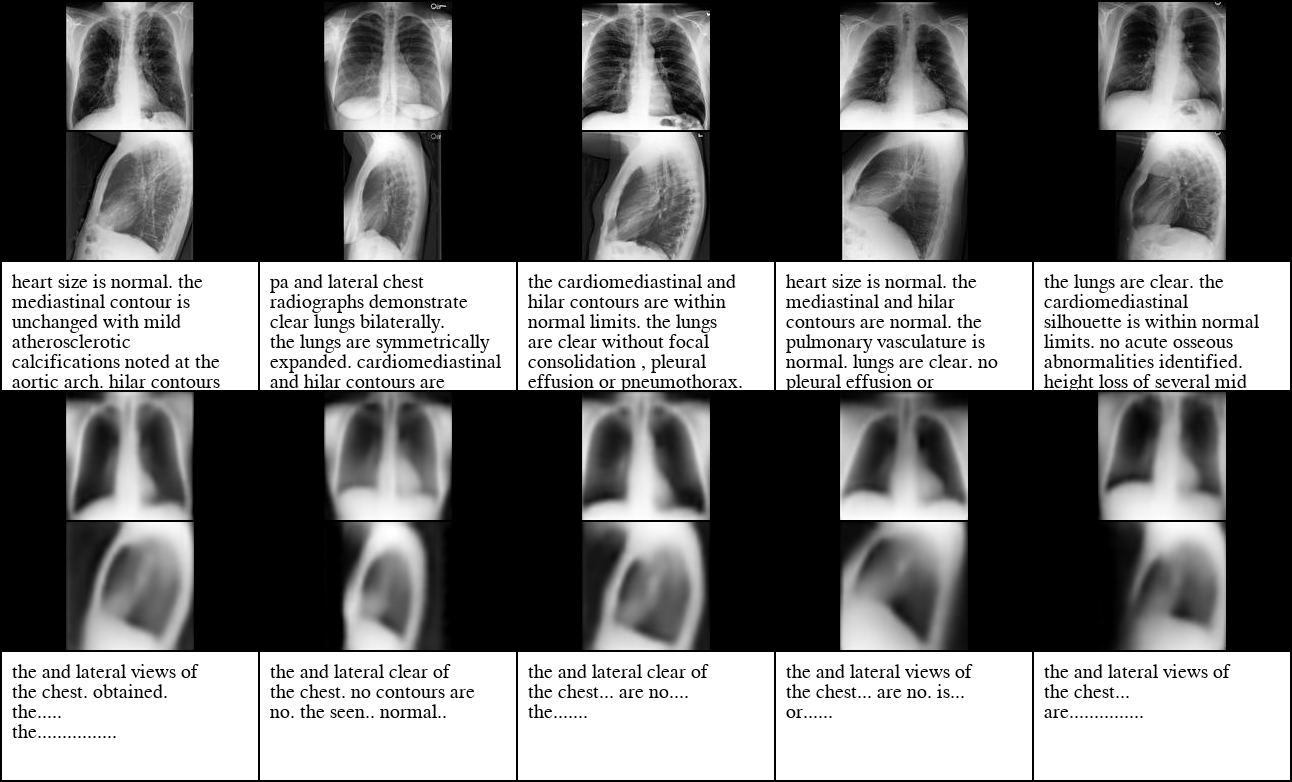
\includegraphics[width=\textwidth]{data/cond_gen/Lateral_PA}
%    \caption{
%        Lateral and PA as conditioner.
%    }
%    \label{fig:fig_cond_latPA}
%\end{figure}
%
%\py{
%    pytex_tab(
%    script='scripts/gen_eval_table.py',
%    label='gen_eval_table',
%    caption='Evaluation of the generation coherence.',
%    options_pre='\\centering \\resizebox{1.1\\textwidth}{!}{',
%    options_post='}',
%    )
%}
%\vspace{0.4em}